% arara: xelatex: { synctex: on, shell: off }
% arara: biber
% arara: xelatex: { synctex: on, shell: off }
% arara: sumatrapdf
\documentclass[12pt, letterpaper]{article}

%Set the document font
\usepackage{fontspec}
\setmainfont[Renderer=Basic,Ligatures=TeX]{Times New Roman}

%Set the size of the margins and the paper
\usepackage[margin=1in, letterpaper]{geometry}

\usepackage{mathtools}

%Set the color of the links and PDF metadata
\usepackage[
    colorlinks=true,
    citecolor=blue,
    linkcolor=black
]{hyperref}

\hypersetup{%
    pdfinfo={
        Title={High Pressure Ignition Chemistry of Alternative Fuels},
        Author={Bryan W. Weber}
    }
}
%Set up the page numbers
%This has to go after geometry so the page number is centered
\usepackage{fancyhdr}
\pagestyle{fancy}
\fancyhf{}
\fancyfoot[C]{\thepage}
\renewcommand{\headrulewidth}{0pt}

%Set a command to easily skip a line
\newcommand{\blankline}{\vspace*{\baselineskip}}

%Set up biblatex
\usepackage[
    backend=biber,
    url=false,
    doi=true,
    sorting=none,
    sortcites=true,
    maxbibnames=6,
    minbibnames=6,
    maxcitenames=2,
    mincitenames=1,
    citestyle=numeric-comp,
    firstinits=true,
    isbn=false
]{biblatex}
\addbibresource{../library.bib}

%Remove the "In:" from before the journal title for articles
\renewbibmacro{in:}{%
  \ifentrytype{article}{}{\printtext{\bibstring{in}\intitlepunct}}}

%Set the sort order of the names in each bibliography entry
\DeclareNameAlias{default}{last-first}

%Don't print the article title. To print the title, add #1 to the last {}
\DeclareFieldFormat[article,incollection,unpublished]{title}{}

%Add Vol. and No. before volume and issue.
\DeclareFieldFormat[article]{volume}{\bibstring{volume}\addspace #1}
\DeclareFieldFormat[article]{number}{\bibstring{number}\addspace #1}

%Put a comma between the volume and issue instead of period
\renewbibmacro*{volume+number+eid}{%
  \printfield{volume}%
  \setunit{\addcomma\space}%<---- was \setunit*{\adddot}%
  \printfield{number}%
  \setunit{\addcomma\space}%
  \printfield{eid}}

%Add a comma after the journal title
\renewbibmacro*{journal+issuetitle}{%
  \usebibmacro{journal}%
  \setunit*{\addcomma\addspace}%
  \iffieldundef{series}
    {}
    {\newunit
     \printfield{series}%
     \setunit{\addspace}}%
  \usebibmacro{volume+number+eid}%
  \setunit{\addspace}%
  \usebibmacro{issue+date}%
  \setunit{\addcolon\space}%
  \usebibmacro{issue}%
  \newunit}

%Set the text to double spacing
\usepackage[doublespacing]{setspace}

%Packages not present in main.tex preamble
\usepackage{booktabs}

\def\chapterautorefname~#1\null{Chap.~#1\null}
\def\sectionautorefname~#1\null{Sec.~#1\null}
\def\subsectionautorefname~#1\null{Sec.~#1\null}
\def\subsubsectionautorefname~#1\null{Sec.~#1\null}
\def\figureautorefname~#1\null{Fig.~#1\null}
\def\tableautorefname~#1\null{Table~#1\null}
\def\equationautorefname~#1\null{Eq.~(#1)\null}

\newcommand{\Autoref}[1]{%
  \begingroup%
  \def\chapterautorefname~##1\null{Chapter~##1\null}%
  \def\sectionautorefname~##1\null{Section~##1\null}%
  \def\subsectionautorefname~##1\null{Section~##1\null}%
  \def\subsubsectionautorefname~##1\null{Section~##1\null}%
  \def\figureautorefname~##1\null{Figure~##1\null}%
  \def\tableautorefname~##1\null{Table~##1\null}%
  \def\equationautorefname~##1\null{Equation~##1\null}%
  \autoref{#1}%
  \endgroup%
}

\usepackage[font={footnotesize}]{caption}

\graphicspath{ {../figures/} }

\usepackage{siunitx}

\usepackage{multirow}

\begin{document}
\section{Rapid Compression Machine}
\label{sec:rcm}
\subsection{Experimental Procedure}
The studies in this dissertation were conducted using the Rapid
Compression Machine (RCM) constructed by Mittal around 2005 and described in the
work of \textcite{Mittal2007,Mittal2006a}. This RCM has been used to
study the autoignition behavior of a number of fuels, including
\textit{n}-decane, methylcyclohexane, hydrogen, syngas,
dimethyl ether, methanol, toluene, benzene, di-isobutylene, iso-octane,
jet fuel, and gasoline \cite{Kumar2009, Mittal2009, Das2012a, Mittal2006,
Das2012, Mittal2008a, Kumar2011a, Mittal2007a, Mittal2008, Kumar2010,
Dooley2010, Dooley2012, Hui2012a, Keromnes2013, Kukkadapu2013, Kukkadapu2012a},
in addition to the studies presented in this work.

A modern RCM operates by rapidly compressing (hence the name) a test gas
mixture to targeted pressure and temperature conditions. The compression
is effected by either a single piston or dual, opposed pistons. Upon
reaching the targeted state, the piston (or pistons) is stopped and
fixed in place so that the reactions proceed in a constant volume
reactor. When studying autoignition with an RCM, the primary data are
the measured pressure traces during and after the compression stroke.
These pressure traces are processed to derive information such as the
pressure and temperature at the end of compression (EOC) and the
ignition delay. It is also possible to employ laser diagnostics or
extract gas samples from the reactor to examine reaction pathways in
more detail.

The present RCM is a pneumatically-driven/hydraulically-stopped
single-piston arrangement. A schematic of the RCM is shown in
\autoref{fig:rcm-schematic}. The RCM consists of four chambers and
three pistons that are used to control machine. The chambers are
called the reaction chamber, the hydraulic chamber, the pneumatic
chamber, and the driving tank; similarly, the pistons are called
the reactor, hydraulic, and pneumatic pistons and are each installed
in the chamber of the same name. The rear of the reaction chamber
is bolted to the front of the hydraulic chamber; seals in the face
of the hydraulic chamber prevent oil from leaking and contaminating
the reaction chamber. The driving tank and the rear of the pneumatic
chamber are connected by a union; a seal around the circumference of
the pneumatic piston seals gas in the driving tank from the front of
the pneumatic chamber. Thus, the pneumatic piston can be driven by
pressure from the driving tank on its rear and pressure from the
pneumatic chamber on its front. The three pistons are connected by
a rod running from the front of the pneumatic piston to the rear of
the reactor piston so that they move as one; this will be referred
to as the piston assembly.

At the start of an experimental run, with the piston in the
EOC position, the reaction chamber is vacuumed to less
than one Torr. Next, the piston assembly is retracted by pressurizing
the front face of the piston in the pneumatic chamber.
For safety, and to prevent damage to the RCM, the driving tank should
be filled to limit the acceleration of the piston assembly during this
retraction.
The pressure on the front of the pneumatic piston pulls the
piston assembly rearward and seats the rear of the
hydraulic piston onto an O-ring in the rear of the
hydraulic chamber. The hydraulic chamber is filled with oil to
a pressure of approximately 800 psi, providing a rearward force on the
front face of the hydraulic piston. Then, the air pressure is released from
the front of the pneumatic chamber and the driving tank is filled to
the desired driving pressure. The
force on the hydraulic piston opposes the force on the pneumatic piston
from the driving tank and the piston assembly remains at rest. Then, the
reaction chamber is filled with the required initial pressure of test
gas mixture from the mixing tank. Finally, compression is triggered by
releasing the hydraulic pressure through an electrically-operated solenoid
valve. The piston assembly is driven forward by the unbalanced force from
the pressure in the driving tank on the pneumatic piston. The gases
in the reaction chamber are brought to the compressed pressure ($P_C$) and
compressed temperature ($T_C$) conditions in approximately 30-50
milliseconds.

The required driving pressure for a given EOC pressure can be estimated
from a force balance between the force on the pneumatic piston from the
driving tank and the force on the reactor piston from the test gases,
as shown in \autoref{eq:driving-pressure}.

\begin{subequations}
\label{eq:piston-force}
\begin{align}
    P_{d,\text{min}} \cdot A_p &= P_{r,\text{EOC}} \cdot A_r \\
    P_{d,\text{min}} \cdot \frac{\pi d_p^2}{4} &= P_{r,\text{EOC}} \cdot \frac{\pi d_r^2}{4} \\
    P_{d,\text{min}} &= P_{r,\text{EOC}} \cdot \frac{d_r^2}{d_p^2} \label{eq:driving-pressure}
\end{align}
\end{subequations}

In \autoref{eq:piston-force}, $P_{d,\text{min}}$ is the minimum
driving pressure, $A_p$ is the cross-sectional area of the pneumatic piston,
$P_{r,\text{EOC}}$ is the pressure in the reactor at the EOC (i.e. $P_C$),
$A_r$ is the cross-sectional area of the reactor piston, $d_p$ is the diameter
of the pneumatic piston, and $d_r$ is the diameter of the reactor piston.

The minimum driving pressure is such that the piston does not rebound at
the EOC due to pressure on the reactor piston. So that the driving
pressure can be much lower than the EOC pressure, the diameter ratio of
the reactor piston to the driver piston is 2/5, allowing a factor of
6.25 lower driving pressure than EOC pressure. The actual driving
pressure should exceed the minimum by some safety margin so that the
reactor remains at constant volume even if there is some pressure rise
due to heat release in the reaction chamber prior to the main ignition.

There is not a theoretical upper limit on the driving pressure. It is desired that the piston should
reach the EOC conditions in as short a time as possible to minimize heat
loss from the reactants to the reactor walls and minimize the time for
reactions to occur during the compression stroke. This implies that the
driving pressure should be made as high as possible so that the highest
piston velocity is achieved. However, higher piston velocities require
a higher deceleration at the EOC. In the present RCM, the deceleration
is provided by venting the hydraulic oil between steps on the hydraulic
piston and matched steps on the front of the hydraulic chamber. If the
piston is overdriven---that is, the driving pressure is too high---the
piston will not be sufficiently decelerated by the oil venting and will
impact the front of the hydraulic chamber at high velocity. This can damage
the RCM and cause the piston to rebound elastically. It also generates
substantial noise in the pressure trace and should be avoided.

Typical driving gas pressures are between 50 psi for $P_C = 15$ bar experiments
to $P_C = 125$ psi for 50 bar experiments. These driving pressures represent a
good compromise between the minimum required for no rebound at EOC due
to pressure and no rebound at EOC due to elastic reaction. Nonetheless,
a small amount of piston rebound can be expected during/after the
main ignition event. This small rebound may have an effect on the computation of
ignition delay if it reduces the pressure rise rate during the ignition;
it is expected that this effect will be very small relative to the
typical random uncertainty in ignition delay experiments. Moreover,
the driving pressures required to balance the full pressure rise during
to ignition are more likely cause elastic rebound,
especially for high $P_C$ when the post-ignition pressure rise is greater.

The EOC conditions ($P_C$ and $T_C$) can be independently varied. This
is made possible by independent variation of the compression ratio,
initial pressure and initial temperature, and the specific heat ratio
of the test gases. The compression ratio can be
increased by adding spacers onto the rear of the hydraulic chamber,
increasing the stroke, and can be reduced by adding split shims onto
the rear of the reaction chamber, increasing the EOC clearance length.

\subsection{Test Gas Mixture Preparation}

Fuel/oxidizer pre-mixtures are prepared in two mixing tanks, one approximately
17 L and the other approximately 15 L in volume. These large volumes allow many
runs to be conducted from one mixture preparation. The mixing tanks are connected
to the reaction chamber by flexible stainless steel manifold tubing. The tanks, reaction chamber,
and connecting manifold are wrapped in heating tape and insulation to control the initial
temperature of the mixture. Temperature controllers from Omega Engineering use thermocouples
placed on the lid of each mixing tank, approximately in the center of each mixing tank, embedded in
the wall of the reaction chamber, and near the inlet valve of the reaction chamber to control the
preheat temperature of the mixture. A static pressure transducer (Omega Engineering, 0-5200 Torr)
measures the pressure in the manifold and mixing tanks. This transducer is used
during mixture preparation and to measure the initial pressure of a given experiment.

Most of the fuels studied in this work are liquids at room temperature and
pressure and have relatively low vapor pressure. A similar procedure, outlined
below, was used for all of the butanol isomers, \textit{iso}-pentanol, and
methylcyclohexane. First, the mixing tanks are vacuumed to an ultimate pressure
less than 5 Torr. The liquid fuel is massed in a syringe to a precision of
0.01 g prior to injection through a septum. Proportions of O$_2$, N$_2$, and
Ar are added manometrically at room temperature. The preheat temperature of
the RCM is set above the saturation point for each fuel to ensure complete
vaporization. The vapor pressure as a function of temperature is calculated
according to fits taken from \textcite{Yaws1999}. A magnetic stirrer mixes
the reactants. The temperature inside the mixing tank is allowed to
equilibrate for approximately 1.5 hours.

This approach to mixture preparation has been validated in several previous
studies by withdrawing gas samples from the mixing tank and analyzing the
contents by GC/MS \cite{Weber2011}, GC-FID \cite{Kumar2009}, and GC-TCD
\cite{Das2012}. These studies have verified the concentration of
\textit{n}-butanol, \textit{n}-decane, and water, respectively. In addition,
both the work by \textcite{Kumar2009} on \textit{n}-decane and the study of
\textcite{Weber2011} on \textit{n}-butanol confirmed that there was no fuel
decomposition over the course of a typical set of experiments. Furthermore,
within this study, each new mixture preparation is checked against previously
tested conditions to ensure reproducibility.

\subsection{Definition of Ignition Delay}
\label{sec:ig-delay-def}

The pressure in the reaction chamber during an experiment is monitored by a
Kistler 6125B piezoelectric dynamic pressure transducer. The charge signal from the
transducer is amplified and converted to a voltage by a Kistler 5010B charge amplifier.
The voltage is sent to a National Instruments cDAQ equipped with the NI-9215 module.
The signal is recorded by a LabView VirtualInstrument at 50 kHz.

\Autoref{fig:ig-delay-def} shows a representative pressure trace from
these experiments with methylcyclohexane (MCH) at $P_C=50$ bar, $T_C=761$ K,
and $\phi=1.5$ (See \autoref{sec:mch}). Note that \autoref{fig:ig-delay-def}
shows a case with two stages of ignition; not all of the fuels studied
had conditions that showed two-stage ignition. Nonetheless, the ignition
delay is consistently defined in all the work in this study. The
definitions of the EOC and the ignition delays are indicated on the figure.
The end of compression time is defined as the time when the pressure
reaches its maximum before first stage ignition occurs, or for cases
where there is no first stage ignition, the maximum pressure before
the overall ignition occurs. The first stage ignition delay is the time
from the end of compression until the first peak in the time derivative
of the pressure. The overall ignition delay is the time from the end of
compression until the largest peak in the time derivative of the pressure.

\begin{figure}
    \centering
    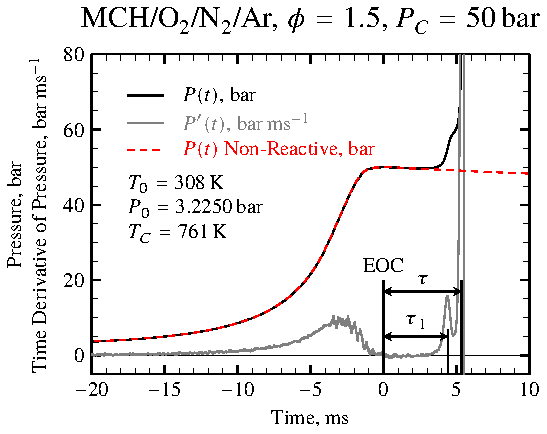
\includegraphics[width=12cm]{02-Experimental-Facilities/ign-delay-def}
    \caption{Representative pressure trace indicating the definition of
    the first stage and overall ignition delays and the corresponding
    non-reactive pressure trace. EOC stands for End of Compression.}
    \label{fig:ig-delay-def}
\end{figure}

Each unique $P_C$ and $T_C$ condition is repeated at least 5 times to
ensure repeatability of the experiments. The experiment closest to the
mean of the runs at a particular condition is chosen for analysis and
presentation. The standard deviation of all of the runs at a condition
is less than 10\% of the mean in all cases.

\subsection{Non-Reactive Experiments}

\Autoref{fig:ig-delay-def} also shows a non-reactive pressure trace.
Due to heat loss from the test mixture to the cold reactor walls,
the pressure and temperature of the gas in the reaction chamber will
decrease after the end of compression. A non-reactive pressure trace
is measured that corresponds to each unique $P_C$ and $T_C$ condition
studied to quantify the effect of the heat loss on the ignition process
and to verify that no heat release has occurred during the compression
stroke. The non-reactive pressure trace is acquired by replacing the
oxygen in the oxidizer with nitrogen, so that the specific heat ratio
of the initial mixture is maintained, but the heat release due to
exothermic oxidation reactions is eliminated. Maintaining a similar
specific heat ratio ensures that the non-reactive experiment faithfully
reproduces the conditions of the reactive experiment. A representative
non-reactive pressure trace is shown in \ref{fig:ig-delay-def}
corresponding to the experimental conditions in the figure.

\subsection{Reaction Chamber Homogeneity}

An RCM to be used for studies of homogeneous chemistry---as in this study---%
must ensure that homogeneous conditions exist inside the reaction
chamber for the duration of the experiment. Due to the high piston
velocities required to minimize heat loss and reaction during the
compression stroke, complex fluid mechanical effects can strongly
affect the state of the reactants at the EOC. The most important of these
effects is caused by the motion of the piston itself, where the piston
pushes the wall boundary layer into a roll-up vortex \cite{Lee1998}.
This cold vortex mixes with the hotter gases near the center of
the reaction chamber and causes large spatial inhomogeneities of
temperature and species.

To facilitate spatially homogeneous conditions in the reactor
and reduce the effect of the roll-up vortex, it is necessary to trap
the boundary layer. This is accomplished on the present RCM by a
crevice machined into the crown of the piston, shown in cross-section
in \autoref{fig:piston}. The boundary layer enters the crevice through
the converging section as the piston moves forward and is trapped
within the crevice. The dimensions of the crevice were optimized
by \textcite{Mittal2006a} through CFD simulations for high-pressure
conditions. Subsequently, \textcite{Mittal2006b} experimentally showed that
the optimized crevice design provides homogeneous conditions in the
reaction chamber up to approximately 150 milliseconds after the EOC.
By using PLIF measurements of acetone-seeded mixtures,
\textcite{Mittal2006b} showed that there was a core region of gases
near the center of the reactor whose temperature remained spatially
homogeneous.

\subsection{Determination of Reactant Temperature}

Two independent thermodynamic properties are required to fix the
thermodynamic state of the reactants in the reaction chamber at a
given time. The first property is the pressure, measured by the dynamic
pressure transducer, as discussed previously; the second property
is chosen to be the temperature.

In general, it is rather difficult to directly measure the temperature
of the gases in the reaction chamber during and after compression.
Intrusive methods such as thermocouples may introduce inhomogeneities into
the reaction chamber and non-intrusive optical techniques are difficult to set up
and require extensive calibration at the pressures of interest in RCM
studies. Thus, the temperature is determined indirectly by applying an
assumption called the "adiabatic core hypothesis" to the reaction chamber
\cite{Mittal2007, Lee1998}.

If all of the gases in the reaction chamber are compressed isentropically,
the temperature at the end of compression can be found by the
following relations:
%
\begin{subequations}
\label{eq:tic}
\begin{align}
\ln\left(\text{CR}\right) = \int_{T_0}^{T_{ic}} \! \frac{1}{T\left(\gamma-1\right)} \, \mathrm{d} T \\
\ln\left(\frac{P_{ic}}{P_0}\right) = \int_{T_0}^{T_{ic}} \! \frac{\gamma}{T\left(\gamma-1\right)} \, \mathrm{d} T
\end{align}
\end{subequations}
%
where CR is the volumetric compression ratio, $T_0$ is the initial temperature,
$T_{ic}$ is the temperature at the end of isentropic compression, $\gamma$ is the
temperature-dependent ratio of specific heats, $P_{ic}$ is the pressure at the
end of isentropic compression, and $P_0$ is the initial pressure.

However, experiments show that the measured pressure in the reaction chamber
does not reach the value of $P_{ic}$ calculated by using the geometric
compression ratio. The difference is due to finite heat loss from the
reactants to the reactor walls and the crevice volume during the
compression. Under the adiabatic core hypothesis, it is assumed that
the heat loss from the reactants only occurs in a thin boundary layer
near the wall, and the central core region is unaffected by heat loss
(i.e. the core is adiabatic) \cite{Desgroux1995}. Thus, the heat
loss is modeled as an effective reduction in the compression ratio, and
the temperature during the compression stroke can be calculated by:
%
\begin{align}
\ln\left(\frac{P_{C}}{P_0}\right) = \int_{T_0}^{T_{C}} \! \frac{\gamma}{T\left(\gamma-1\right)} \, \mathrm{d} T
\label{eq:tc}
\end{align}
%
where $P_C$ is the measured pressure at the end of compression, $T_C$
is the temperature at the end of compression, and the other variables
are the same as in \autoref{eq:tic}.

After the end of compression, the pressure in the reaction chamber
decreases, as can be seen in \autoref{fig:ig-delay-def}. This pressure
decrease is caused by heat loss from the reactants in the constant volume reaction
chamber and is accompanied by a decrease in the temperature of the
reactants. To model the thermodynamic state after the end of compression,
the adiabatic core hypothesis is applied, and the heat loss is
assumed to occur only in a thin boundary layer near the reactor walls.
Thus, the core region is modeled as adiabatic, and the heat loss
from the boundary layer can be modeled as an isentropic volume
expansion.

\subsection{Determination of Compressed Temperature}

In general, the specific heat ratio used in Eqs. (\ref{eq:tic}) and
(\ref{eq:tc}) is a function of temperature and composition, so \autoref{eq:tc} cannot
be integrated directly to find $T_C$. If the specific heats are parameterized with a
linear fit, it is possible to integrate \autoref{eq:tc} directly,
but this process is quite tedious; nonetheless, it will be applied in
\autoref{sec:uncertainty} to determine the uncertainty of $T_C$. In
general, the simplest method of calculating $T_C$ is to use software
numerically integrate \autoref{eq:tc}.

In this work, the CHEMKIN-Pro \cite{Chemkin2012} software is used to
perform the numerical integration and calculation of $T_C$. The
CHEMKIN-Pro software provides the facility for a user-specified
volume as a function of time to be applied to a homogeneous,
adiabatic reactor. Since the adiabatic core of the reaction chamber
is modeled as undergoing an isentropic volumetric compression followed
by an isentropic volumetric expansion, the user-specified volume
functionality is used to compute the RCM reactor state as a function
of time. A volume trace for simulation is computed from the measured
pressure trace using the isentropic relation:
%
\begin{align}
\frac{V_2}{V_1} = \left[\frac{P_1}{P_2}\right]^{\frac{1}{\gamma}}
\label{eq:volume-trace}
\end{align}
%
where $V_1$ and $V_2$ are the volumes at consecutive time points,
$P_1$ and $P_2$ are the pressures at consecutive time points, and
$\gamma$ is the temperature dependent specific heat. This equation
is applied during and after the compression stroke to calculate
the volume trace. In \autoref{eq:volume-trace} it is assumed that
changes in composition of the reactants are negligible during the
compression stroke.

For use in \autoref{eq:volume-trace}, $\gamma$ is tabulated for each
time point. Thus, the temperature at each time point must also be
computed by using the isentropic relation for temperature:
%
\begin{align}
\frac{T_2}{T_1} = \left[\frac{P_2}{P_1}\right]^{\frac{\gamma-1}{\gamma}}
\label{eq:isen-temp}
\end{align}
%
where $T_2$ and $T_1$ are the temperatures at consecutive time points.
Since $T_2$ depends on the value of $\gamma$, which in turn depends
on $T_2$, \autoref{eq:isen-temp} is iterated until the temperature
changes by less than one tenth of one percent on consecutive iterations.
Once again, it is assumed that changes in composition have a negligible
influence on the ratio of specific heats.
The temperature calculated by \autoref{eq:isen-temp} is typically within
1K of the temperature calculated by CHEMKIN-Pro.

\subsection{Uncertainty of Ignition Delay and Compressed Temperature}
\label{sec:uncertainty}

The uncertainty of the compressed temperature is an important parameter
to report. Since $T_C$ is not measured, we must perform an uncertainty
propagation analysis on the equation used to calculate $T_C$,
\autoref{eq:tc}. First, we simplify the term involving $\gamma$ in
\autoref{eq:tc}. By definition, $\gamma$ is the ratio of the specific heat
at constant pressure to that at constant volume
%
\begin{align}
\gamma = \frac{C_p}{C_v} = \frac{C_p/R}{C_v/R}
\end{align}

where $C_p$ and $C_v$ are the specific heats in molar units at constant
pressure and volume, respectively, and $R$ is the universal gas constant,
used to produce non-dimensional specific heats. Letting a hat denote the
non-dimensional specific heats, the difference between the non-dimensional
specific heats is one, $\hat{C}_v = \hat{C}_p - 1$. Then, it follows that
%
\begin{align}
\label{eq:simplify-gamma}
\frac{\gamma}{\gamma - 1} = \frac{\frac{\hat{C}_p}{\hat{C}_v}}{\frac{\hat{C}_p}{\hat{C}_v} - 1}
= \frac{\frac{\hat{C}_p}{\hat{C}_p - 1}}{\frac{\hat{C}_p}{\hat{C}_p - 1} - 1}
= \frac{\frac{\hat{C}_p}{\hat{C}_p - 1}}{\frac{1}{\hat{C}_p - 1}}
= \hat{C}_p
\end{align}

In \autoref{eq:tc}, the mean specific heat ratio for the mixture
should be used; thus, the simplification as shown in \autoref{eq:simplify-gamma}
requires that the specific heat $\hat{C}_p$ also be the mean specific
heat. In the following, we assume that there is negligible
change of the mean specific heat due to changes in reactant
mole fractions. The mean specific heat is simply the sum of the product of
the species mole fractions and their specific heats
%
\begin{subequations}
\label{eq:cp}
\begin{align}
C_{p\text{,total}} &= \sum_i X_i C_{p,i} \\
\hat{C}_{p\text{,total}} &= \frac{\sum_i X_i C_{p,i}}{R}
\end{align}
\end{subequations}
%
where $i$ indicates the species and $X_i$ is the species mole fraction.
In the NASA polynomial formulation used by CHEMKIN, the non-dimensional specific
heat at constant pressure as a function of temperature is represented by a
fourth-order polynomial fit
%
\begin{align}
\hat{C}_{p,i} = c_{1,i} + c_{2,i} T + c_{3,i} T^2 + c_{4,i} T^3 + c_{5,i} T^4
\end{align}
%
In general, this means that the specific heat can be non-linear. However,
the mixtures prepared in this study are composed primarily of
O$_2$, N$_2$ and Ar (i.e. no more than 5\% of any mixture is the
fuel), and the specific heats of O$_2$, N$_2$ and Ar are only weakly
temperature dependent over the range of temperatures experienced during
compression, we will approximate the total specific heat as a linear function
of temperature.
%
\begin{equation}%
\label{eq:cp-total}
\begin{split}
\hat{C}_{p\text{,total}} &= \sum_i X_i \hat{C}_{p,i} \\
&= \sum_i X_i \left( \sum_{j=1}^5 c_{j,i} T^{j-1} \right) \\
&\approx a + b T
\end{split}
\end{equation}
%
$a$ and $b$ are found by fitting the total non-dimensional specific heat
over the temperature range from 300--1100 K, as discussed below in
\autoref{sec:unc-cp}.

With this approximation of the specific heat, we can integrate \autoref{eq:tc}
to find the compressed temperature
%
\begin{subequations}
\begin{align}
\ln{\frac{P_C}{P_0}} &= \int_{T_0}^{T_{C}} \! \frac{\gamma}{T\left(\gamma-1\right)} \, \mathrm{d} T
                      = \int_{T_0}^{T_{C}} \! \frac{\hat{C}_p}{T} \, \mathrm{d} T \\
&= \int_{T_0}^{T_{C}} \! \frac{a + b T}{T} \, \mathrm{d} T\\
&= a \ln{T} + b T \Big|_{T_0}^{T_C}
\end{align}
\begin{equation}
\ln{\frac{P_C}{P_0}} = a \ln{T_C} + b \ln{T_C} - \left(a \ln{T_0} + b T_0\right) \label{eq:integrate-tc}
\end{equation}
\end{subequations}

Using a computer algebra system, \autoref{eq:integrate-tc} can be solved for $T_C$
%
\begin{align}
\label{eq:explicit-tc}
T_C = \frac{a W\!\!\left(\frac{b}{a} \exp\!{\left[\frac{b T_0}{a}\right]} T_0 \left[\frac{P_C}{P_0}\right]^{\frac{1}{a}}\right)}{b}
\end{align}
%
where $W(...)$ is Lambert's W function. With an explicit function for $T_C$, we can
estimate the uncertainty in $T_C$ by the root square sum of the uncertainty in the parameters in
\autoref{eq:explicit-tc} \cite{Taylor1982}. The parameters are $P_C$, $P_0$, $T_0$, $a$, and $b$.
%
\begin{align}
\label{eq:tc-unc}
U_{T_C} = \sqrt{\left(\frac{\partial T_C}{\partial P_C} U_{P_C}\right)^2 + \left(\frac{\partial T_C}{\partial P_0} U_{P_0}\right)^2 +
                \left(\frac{\partial T_C}{\partial T_0} U_{T_0}\right)^2 + \left(\frac{\partial T_C}{\partial a} U_{a}\right)^2 +
                \left(\frac{\partial T_C}{\partial b} U_{b}\right)^2}
\end{align}

Once again using a computer algebra system, we find the partial derivatives of
\autoref{eq:explicit-tc} with respect to the parameters. Letting
%
\begin{equation*}
D = W\!\!\left(\frac{b}{a} \exp\!{\left[\frac{b T_0}{a}\right]} T_0 \left[\frac{P_C}{P_0}\right]^{\frac{1}{a}}\right)
\end{equation*}
%
the terms are
%
\begin{subequations}
\begin{align}
\frac{\partial T_C}{\partial P_C} &= \frac{D}{b P_C \left(D + 1\right)} \\
\frac{\partial T_C}{\partial P_0} &= \frac{-D}{b P_0 \left(D + 1\right)} \\
\frac{\partial T_C}{\partial T_0} &= \frac{\left(a + b T_0\right) D}{b T_0 \left(D + 1\right)} \\
\frac{\partial T_C}{\partial a} &= \frac{-D \left[b T_0 + \ln{\left(P_C/P_0\right)} - a D\right]}{a b \left(D + 1\right)} \\
\frac{\partial T_C}{\partial b} &= \frac{D\left(b T_0 - a D\right)}{{b}^2\left(D + 1\right)}
\end{align}
\end{subequations}

The uncertainties of the parameters, $U_j$ in \autoref{eq:tc-unc}, are in
general found by their own root square sum procedure.
%
\begin{align}
{U_j}^2 = {B_j}^2 + {R_j}^2
\end{align}
%
where the subscript $j$ represents one of the parameters in \autoref{eq:explicit-tc}.
The total uncertainty of a particular parameters is composed of
two parts, the systematic or bias uncertainty ($B_j$) and the
precision or random uncertainty ($R_j$). In general, the bias
uncertainty is contained in the measurement equipment and can
be reduced, e.g. by using different equipment; the random uncertainty
is inherent in any measured process and cannot be reduced by
experimental techniques. The bias and precision uncertainties
for each parameter will be discussed in the following.

\subsubsection{Uncertainty in Initial Temperature}

The bias uncertainty in the initial temperature is due to the standard
limits of error of the K-type thermocouple used to measure the
initial temperature. According to the Omega Engineering
specifications, this is "the greater
of $\SI{2.2}{\degreeCelsius}$ or 0.75\%". The largest initial temperatures
used in this work, 413 K, lead to an uncertainty of
$\pm \SI{3}{\kelvin}$; thus, $B_{T_O}=\SI{3}{K}$. Bias uncertainty
due to the A/D converter in the process meter is negligible compared
to this uncertainty.
The precision uncertainty is due to the limit of precision of
the display on the Omega Engineering CNi3254 process meter used
to control the process temperature. This is $\pm\SI{0.5}{K}$.
The total uncertainty of the initial temperature is
%
\begin{align}
U_{T_0} = \sqrt{\left(B_{T_0}\right)^2 + \left(R_{T_0}\right)^2} = \sqrt{\left(\SI{3}{K}\right)^2 + \left(\SI{0.5}{K}\right)^2} = \SI{3.04}{K}
\end{align}

\subsubsection{Uncertainty in Initial Pressure}
\label{sec:unc-p0}

The bias uncertainty in the initial pressure is due to the
standard error in the pressure transducer used to measure
the initial pressure. Two different pressure transducers have
been used in this study; the first, an Omega Engineering PX-303
(range: 0--\SI{50}{psia}), has a full scale uncertainty of 1.25\%, or
$\pm \SI{0.625}{psi} \ (\SI{4309.2}{Pa})$. The second transducer is an
Omega Engineering MMA100V10T2D0T4A6 type (range: 0--\SI{5200}{Torr}) and was
purchased because preliminary results of this uncertainty analysis
indicated that the largest contributor to the uncertainty of $T_C$ was
the initial pressure measurement. The full scale uncertainty of the MMA
type transducers is 0.05\%, resulting in an uncertainty of
$\pm \SI{2.6}{Torr} \ (\SI{346.6}{Pa})$, an order of magnitude lower than
the PX-303 while also providing more than double the operating range. Total
uncertainties using the appropriate pressure transducer are reported in
each experimental section of this work; both transducers will be analyzed
in this section. Bias uncertainty due to the signal acquisition equipment
is negligible compared to the standard error in the pressure transducers.

The precision uncertainty is due to the limit of precision of the display
on the Omega Engineering DP41-B process meter used to monitor the initial
pressure. This is $\pm\SI{0.005}{torr} \ (\SI{0.666}{Pa})$. The total
uncertainty of the initial pressure is
%
\begin{subequations}
\begin{align}
U_{P_0} = \sqrt{\left(B_{P_0}\right)^2 + \left(R_{P_0}\right)^2} = \sqrt{\left(\SI{4309.2}{Pa}\right)^2 + \left(\SI{0.666}{Pa}\right)^2} = \SI{4309.2}{Pa} \\
U_{P_0} = \sqrt{\left(B_{P_0}\right)^2 + \left(R_{P_0}\right)^2} = \sqrt{\left(\SI{346.6}{Pa}\right)^2 + \left(\SI{0.666}{Pa}\right)^2} = \SI{346.6}{Pa}
\end{align}
\end{subequations}

\subsubsection{Uncertainty in Compressed Pressure}

The bias uncertainty in the compressed pressure is due to the standard
error in the piezoelectric pressure transducer. According to the
manufacturer calibration, the deviation of the full scale output from
linearity is less then 0.2\%, indicating that $B_{T_C}=\SI{0.5}{bar}$.
The uncertainties in the signal acquisition equipment are negligible
compared to this uncertainty. The precision uncertainty is due to the limit
of precision of the output of the pressure, and is \SI{5E-7}{bar}. This
is negligible compared to the bias uncertainty, so the total uncertainty
of the compressed pressure is
%
\begin{equation}
U_{P_C} = B_{T_C} = \SI{0.5}{bar}
\end{equation}

\subsubsection{Uncertainty in the Specific Heat}
\label{sec:unc-cp}

The uncertainty in the specific heat comes from two sources. First is the
uncertainty in the mixture composition and second is the uncertainty in
the linear fit to the total specific heat. The uncertainty in the mixture
composition can be estimated by the same method as is used for $T_C$. The
specific heat is given by \autoref{eq:cp}, so we can take partial derivatives
of that equation with respect to the mole fractions of the species to find
the total uncertainty
%
\begin{equation}
\label{eq:cp-uncertainty}
\begin{split}
\left(U_{\hat{C}_{p\text{,total}}}\right)^2 &= \left(\frac{\partial \hat{C}_p}{\partial X_1} U_{X_1}\right)^2 + \ldots + \left(\frac{\partial \hat{C}_p}{\partial X_n} U_{X_n}\right)^2 \\
&= \left(\hat{C}_{p,1} U_{X_1}\right)^2 + \ldots + \left(\hat{C}_{p,n} U_{X_n}\right)^2
\end{split}
\end{equation}
%
where $n$ is the total number of species. In \autoref{eq:cp-uncertainty},
it is assumed that the uncertainty in the specific heats of each species
is negligible. This is considered an acceptable assumption for stable species
such as the fuel molecules, oxygen, nitrogen, and argon. Experience with
several kinetic mechanisms has shown that the typical variation in individual
$\hat{C}_p$ fits causes approximately $\mathcal{O}(\SI{1}{K})$ changes in $T_C$.

The uncertainty of the mole fraction of the species is estimated differently
depending on how the species was introduced to the mixing tank. For liquid fuel
species, experiments with GC/MS have shown that there is approximately 5\%
variation in mole fraction from the expected value \cite{Weber2011}; this value is adopted for
the total uncertainty of all liquid fuels. The mole fraction of the gaseous species
is determined by their partial pressures when filling; the mole fraction is
related to the pressure by Dalton's Law of Partial Pressure
\cite{Dalton1801,Gillespie1930}
%
\begin{equation}
X_i = \frac{P_i}{P}
\end{equation}
%
where $P_i$ is the partial pressure of a species and $P$ is the total pressure.
It follows that
%
\begin{equation}
\begin{split}
\left(U_{X_i}\right)^2 &= \left(\frac{\partial X_i}{\partial P_i} U_{P_i}\right)^2 + \left(\frac{\partial X_i}{\partial P} U_P\right)^2 \\
&= \left(\frac{U_{P_i}}{P}\right)^2 + \left(\frac{{-P_i}}{P^2} U_P\right)^2
\end{split}
\end{equation}
%
The uncertainty of the pressures $P_i$ and $P$ can be estimated by
the same procedure as in \autoref{sec:unc-p0} since the same pressure transducer
is used to measure the pressure. A typical total pressure after filling is
approximately \SI{2000}{Torr} ($\approx$ \SI{266644}{Pa}). The mixtures in
\autoref{tab:mixtures} are the mixtures that will be analyzed in the
following because they represent a worst case scenario in that the mole
fraction of the fuel or oxygen is maximized in them.

\begin{table}
\centering
\caption{Mixtures studied in the uncertainty analysis.}
\label{tab:mixtures}
\begin{tabular}{l *{4}{c}}
    \toprule
    \multirow{2}[0]{*}{Fuel} & \multicolumn{4}{c}{Mole Fraction} \\
         & Fuel & Oxygen & Nitrogen & Ar \\
    \midrule
    Methylcyclohexane   & 0.0107 & 0.2240 & 0.0000 & 0.7653 \\
    \textit{n}-Butanol  & 0.0676 & 0.2030 & 0.7294 & 0.0000 \\
    \textit{i}-Pentanol & 0.0531 & 0.1989 & 0.7480 & 0.0000 \\
    Propene             & 0.0854 & 0.1921 & 0.7225 & 0.0000 \\
    \bottomrule
    \end{tabular}
\end{table}

Once the total specific heat has been calculated, a linear fit as a function
of temperature is applied by least-squares estimation. Since there is an uncertainty
in the specific heat, there is a corresponding uncertainty in the fit
coefficients $a$ and $b$. Following the methodology outlined by
\textcite{York2004}, the values and uncertainties of $a$ and $b$
are calculated iteratively. This procedure gives identical values of the
slope, intercept, and standard errors as maximum likelihood estimation \cite{York2004}.
\Autoref{eq:york} is reproduced from \textcite{York2004}, and is presented
as Eq. (13) in that work.
%
\begin{subequations}
\label{eq:york}
\begin{align}
a &= \overline{Y} - b\overline{X}  \label{eq:intercept}\\
b &= \frac{\sum W_i \beta_i V_i}{\sum W_i \beta_i U_i} \label{eq:slope}\\
\sigma_a^2 &= \frac{1}{\sum W_i} + \overline{x}^2\sigma_b^2 \label{eq:unc-intercept}\\
\sigma_b^2 &= \frac{1}{\sum W_i u_i^2} \label{eq:unc-slope}
\end{align}
\end{subequations}
%
where the symbols in \autoref{eq:york} are defined in \autoref{tab:york-syms}.
The general formulation is given here because it will be reused in
\autoref{sec:unc-gcms}; application to this section will
be given below.

\begin{table}
\centering
\caption{Symbols in \autoref{eq:york}. Reproduced from the work of \textcite{York2004}.}
\label{tab:york-syms}
\begin{tabular}{ll}
\toprule
Symbol & Meaning \\
\midrule
$a$, $b$ & $y$ intercept and slope of best line, $y=a+b x$ \\
$\sigma_a$, $\sigma_b$ & Standard errors of $a$ and $b$ \\
$X_i$, $Y_i$ & Calculated total specific heat for a given temperature \\
$x_i$, $y_i$ & Least-squares adjusted points \\
$\omega(X_i)$, $\omega(Y_i)$ & Weights of $X_i$ and $Y_i$ \\
\addlinespace
$\alpha_i$ & $\sqrt{\omega(X_i)\omega(Y_i)}$ \\
\addlinespace
$r_i$ & Correlation coefficient between uncertainty in $X_i$ and $Y_i$ \\
\addlinespace
$W_i$ & $\dfrac{\omega(X_i)\omega(Y_i)}{\omega(X_i) + b^2\omega(Y_i) - 2br_i\alpha_i}$ \\
\addlinespace
$\overline{X}$, $\overline{Y}$ & $\dfrac{\sum W_i X_i}{\sum W_i}$, $\dfrac{\sum W_i Y_i}{\sum W_i}$ \\
\addlinespace
$U_i$, $V_i$ & $X_i - \overline{X}$, $Y_i - \overline{Y}$ \\
\addlinespace
$\overline{x}$ & $\dfrac{\sum W_i x_i}{\sum W_i}$ \\
\addlinespace
$\beta_i$ & $W_i \left[\dfrac{U_i}{\omega(Y_i)} + \dfrac{bV_i}{\omega(X_i)} - \left(bU_i + V_i\right)\dfrac{r_i}{\alpha_i}\right]$ \\
\addlinespace
\bottomrule
\end{tabular}
\end{table}

In this section, $X_i$ are the temperatures at which \autoref{eq:cp-total}
is evaluated and $Y_i$ are the total specific heats evaluated from \autoref{eq:cp-total}.
The weighting of the specific heats---$\omega(Y_i)$---is taken
to be the reciprocal of the uncertainty as calculated by
\autoref{eq:cp-uncertainty}. Furthermore, there is no uncertainty in the
abscissa (i.e. the temperature) and $\omega(X_i) = 1$. Finally, since there
is no uncertainty in the temperature, there is no correlation between
the uncertainties, i.e. $r_i = 0$.

First, the slope $b$ is estimated by simple least-squares regression of the total
specific heat on the temperature. Then, this slope is used to estimate the
adjusted weighting of each point, $W_i$. Next, $U_i$ and $V_i$ are calculated
based on the adjusted weighting. Using $U_i$, $V_i$, and $\beta_i$, a new value of the
slope is calculated from \autoref{eq:slope}, and the process is repeated until the slope converges.
Convergence is determined when the slope changes by less than 0.001 on successive
iterations. Then, using \autoref{eq:intercept}, the intercept $a$ is calculated.
Finally, the standard error of each parameter is
calculated using the final values of the slope and intercept with Eqs. (\ref{eq:unc-slope})
and (\ref{eq:unc-intercept}).

For the mixtures considered in
this study, the correlation coefficient for the linear fits are greater than
0.99 (i.e. $r^2 > 0.99$), indicating a good fit.
\end{document}
